There are several ways to combine two existing functions to create a new function.  In this section, we will focus on one way, the composition of two functions.  We will also consider some results about the compositions of injections and surjections.

\subsection*{Composition of Functions}
The basic idea of function composition is that when possible, the output of a function  $f$  is used as the input of a function  $g$.  This can be referred to as ``$f$  followed by  $g$'' and is called the composition of  $f$  and  $g$. 

The idea of the composition of two real functions is familiar from previous mathematics courses.  For example, if  $f( x ) = 3x^2  + 2$ and  
$g( x ) = \sin x$, then we can compute  $g( {f( x )} )$
 as follows:
\[
\begin{aligned}
  \hfill g( {f( x )} ) &= g \! \left( {3x^2  + 2} \right) \\
                       &= \sin \! \left( {3x^2  + 2} \right). \\ 
\end{aligned} 
\]
In this case,  $f( x )$, the output of the function  $f$, was used as the input for the function  $g$.  This idea of using the output from one function as the input for another function can be illustrated nicely with arrow diagrams.  This was done in Preview Activity~\ref{PA:compositionintro}, and another example is given here.

Let  $A = \left\{ {a, b, c, d} \right\}$, $B = \left\{ {p, q, r} \right\}$, and  
$C = \left\{ {s, t, u, v} \right\}$.  The arrow diagram in Figure~\ref{fig:arrow64-1} shows two functions:  
$f\x A \to B$  and  $g\x B \to C$.
\begin{figure}[h]
\begin{center}
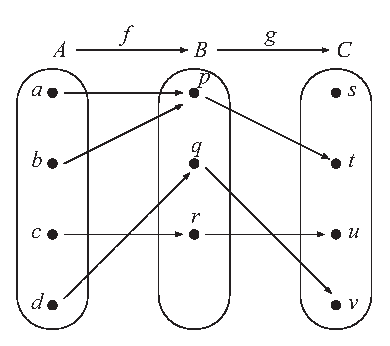
\includegraphics{figps-sec641.eps} 
\caption{Arrow Diagram for Two Functions} \label{fig:arrow64-1}
\end{center}
\end{figure}

If we follow the arrows from the set  $A$  to the set  $C$, we will use the outputs of  $f$  as inputs of  $g$, and get the arrow diagram from  $A$  to  $C$ shown in Figure~\ref{fig:arrow64-2}.  This diagram represents the composition of  $f$  and  $g$  and is denoted by  $g \circ f$\!.
\begin{figure}[h]
\begin{center}
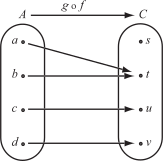
\includegraphics{figps-sec642.eps} 
\caption{Arrow Diagram for $g \circ f\x  A \to C$} \label{fig:arrow64-2}
\end{center}
\end{figure}
%
\begin{defbox}{functioncomposition}{Let  $A$, $B$, and  $C$  be nonempty sets, and let  
$f\x A \to B$  and  $g\x B \to C$  be functions.  The \textbf{composition of}
\index{composition of functions}%
\index{function!composition}%
  $\boldsymbol{f}$ \textbf{and} $\boldsymbol{g}$  is the function  $g \circ f\x A \to C$  defined by
\label{sym:composition}
\[
( {g \circ f} )( x ) = g\left( {f( x )} \right)
\]
for all  $x \in A$.  We often refer to the function  $g \circ f$ as a \textbf{composite function}.
\index{function!composite}%
\index{composite function}%
}
\end{defbox} 
%
It is helpful to think of the composite function  $g \circ f$
 as  ``$\boldsymbol{f}$  \textbf{followed by}  $\boldsymbol{g}$.''  We then refer to  $f$  as the \textbf{inner function}
\index{inner function}%
\index{composition of functions!inner function}%
 and  $g$  as the \textbf{outer function}.
\index{outerfunction}%
\index{composition of functions!outer function}%


\endinput
